
\documentclass[11pt,a4paper]{article}
\usepackage[utf8]{inputenc}
%\usepackage[icelandic]{babel}
%\usepackage[T1]{fontenc}
\usepackage{amsmath}
\usepackage{amsfonts}
\usepackage{amssymb}
%\usepackage{graphicx}
%\author{Arnar Ingi Halldórsson}
%\title{Linear Motion}


%\documentclass{article}
\usepackage{graphicx}
\graphicspath{ {myndir/} }
\usepackage[T1]{fontenc} 
\usepackage[english]{babel}

\usepackage[utf8]{inputenc} 
\usepackage{graphics}
%\usepackage[pdftex]{graphicx}

\usepackage{caption}
\usepackage{subcaption}

\usepackage{titling}

\setlength{\droptitle}{-10em}
   
\title{Assignment 1 \\ T-509-RAFT \\ Electronics} % Title

\author{Arnar Ingi Halldórsson \\ Hjörleifur G Bergsteinsson \\ Snorri Stefánsson} % Author name
\begin{document}

\maketitle % Insert the title, author and date

\begin{tabular}{lr}
Due date: 22.02.2015 \\
Teachers:\qquad Slawomir Koziel\\ % Instructor/supervisor
\qquad \qquad \qquad Adrian Bekasiewicz
\end{tabular}

\setlength\parindent{0pt} % Removes all indentation from paragraphs

\renewcommand{\labelenumi}{\alph{enumi}.} % Make numbering in the enumerate environment by letter rather than number (e.g. section 6)

\section*{Introduction}


\section*{Task 1: Perfomance Parameters of Op Amp}

\begin{enumerate}
  \item[1.]
		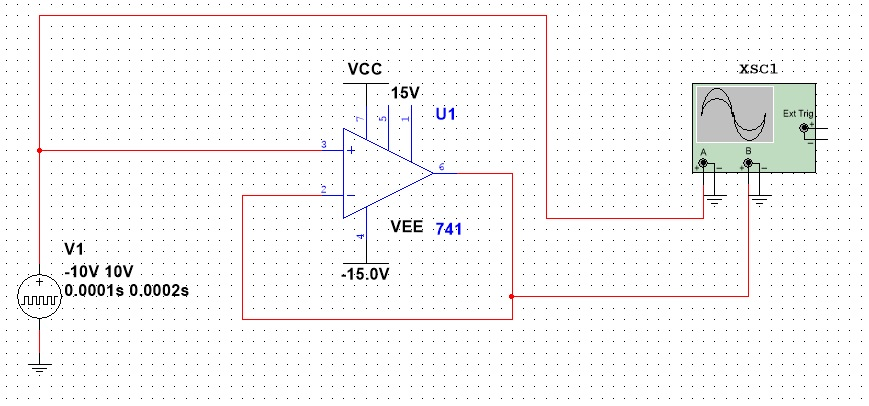
\includegraphics[width=10cm]{Task1-1Circuit}\\
		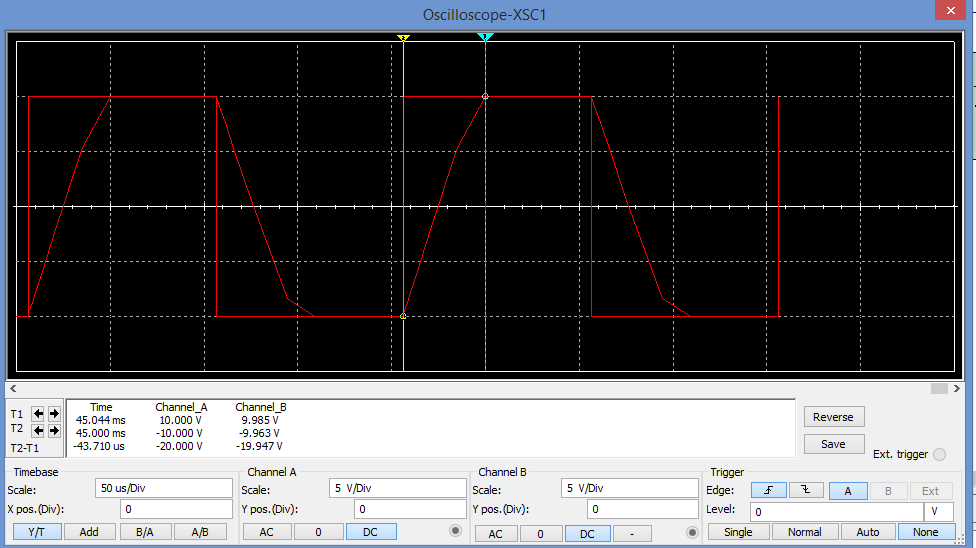
\includegraphics[width=10cm]{Task1-1-Oscilloscope}
  
  \item[2.]
  		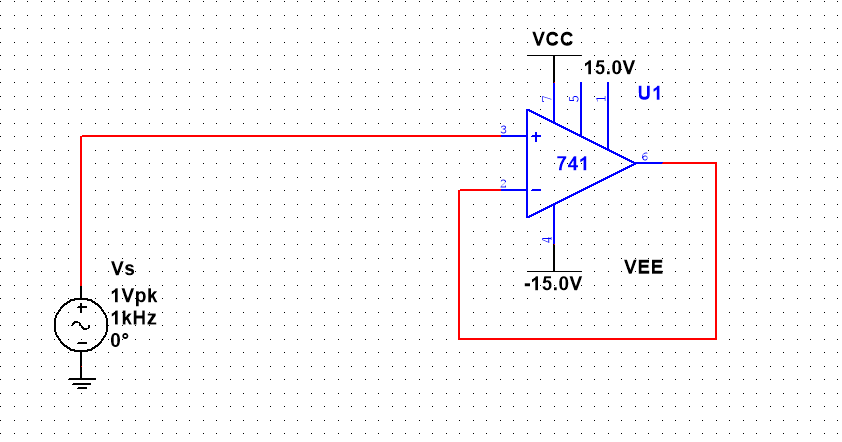
\includegraphics[width=10cm]{Task1-2-Circuit}\\
		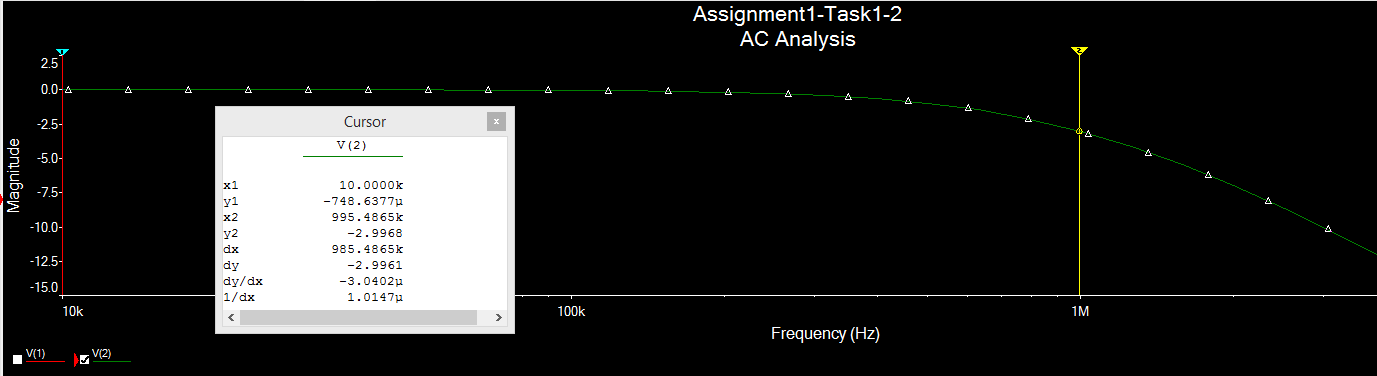
\includegraphics[width=10cm]{Task1-2-ACAnalysis}
  \item[3.]
    	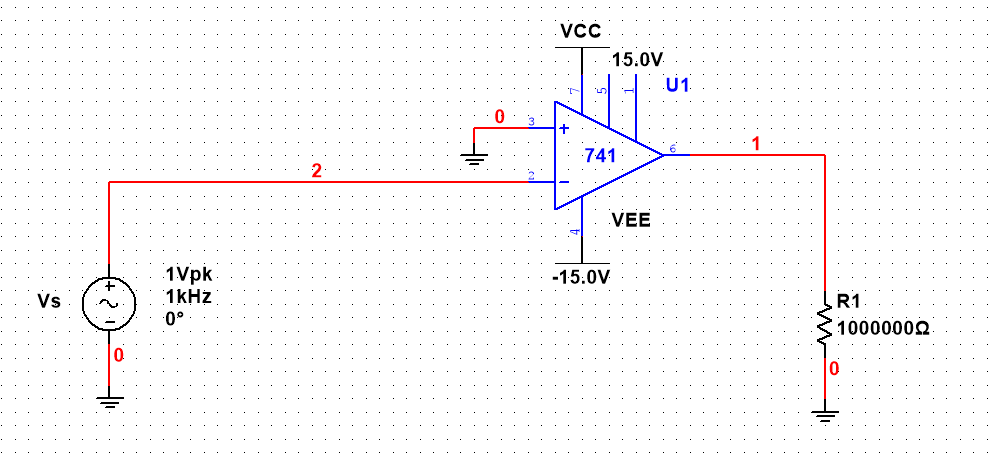
\includegraphics[width=10cm]{Task1-3-Circuit}\\
		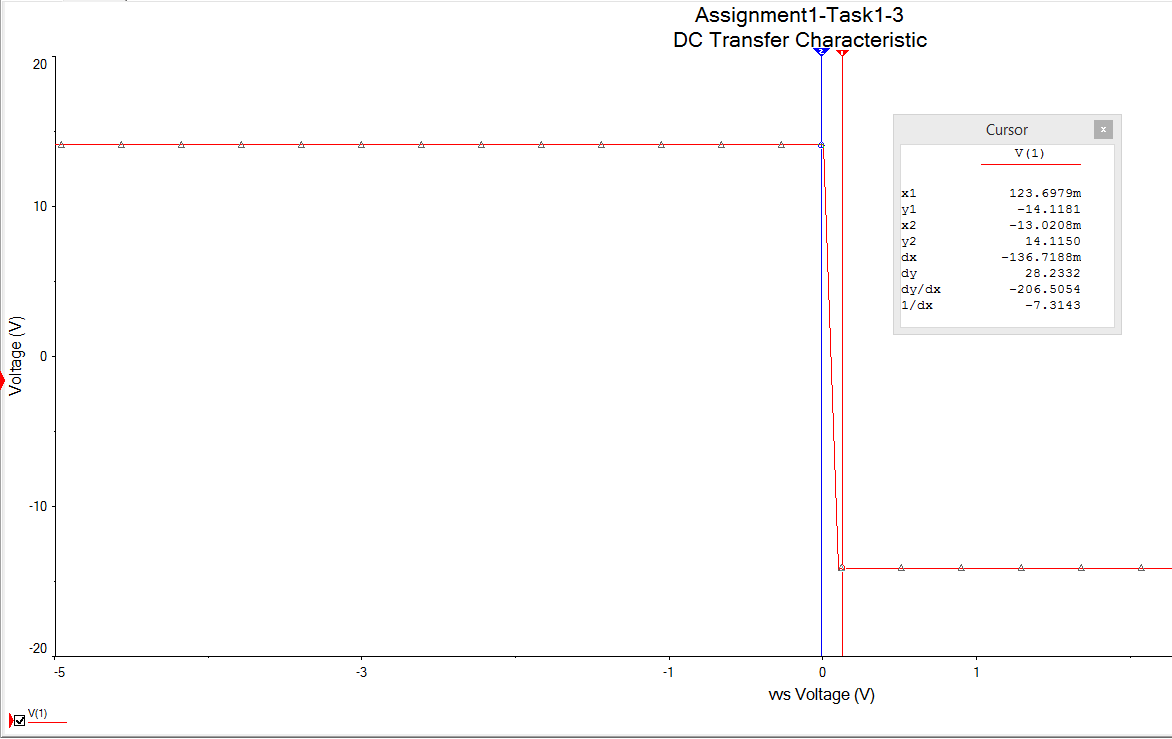
\includegraphics[width=10cm]{Task1-3-DCAnalysis}
  \item[4.]
  
	\begin{tabular}{l*{3}{c}r}
	$\mu$ A741 op-Amp              & DataSheet & Simulation  \\
	\hline
	Slew Rate [$SR$]   & 6 & 4 \\
	Gain-Bandwidth [$GBW$]              & 6 & 3 \\
	DC Differential Gain [$A_{d}$]             & 6 & 2 \\
	Input Offset Voltage [$V_{os}$]           & 6 & 2 \\
	\end{tabular}

\end{enumerate}

\section*{Task 2: Frequency Response of Inverting Amplifier}

\begin{enumerate}
  \item[1.]
  
  \item[2.]
  
\end{enumerate}

\section*{Task 3: Op Amplifies Design}

\begin{enumerate}
  \item[1.]
  
  \item[2.]
  
  \item[3.]
  
\end{enumerate}

\section*{Task 4: Half - Wave Rectifier}

\begin{enumerate}
  \item[$\bold{1.}$]
  Here is the half-wave rectifier circuit:
  \\
  
	\begin{minipage}{\linewidth}
    	\centering
		\captionof{figure}{}        
        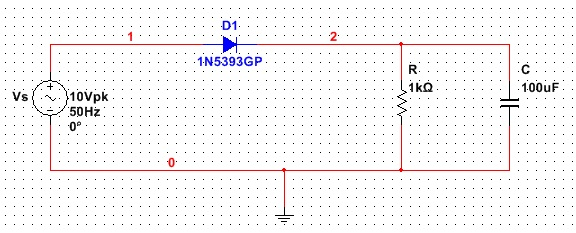
\includegraphics[width=13cm]{4_1.jpg}
    \end{minipage}
    
  
  \item[$\bold{2.}$]
  Now lets do a transient analysis of the circuit:
  \\
	\begin{minipage}{\linewidth}
    	\centering
		\captionof{figure}{Transient analysis of circuit the circuit in the last figure.}        
        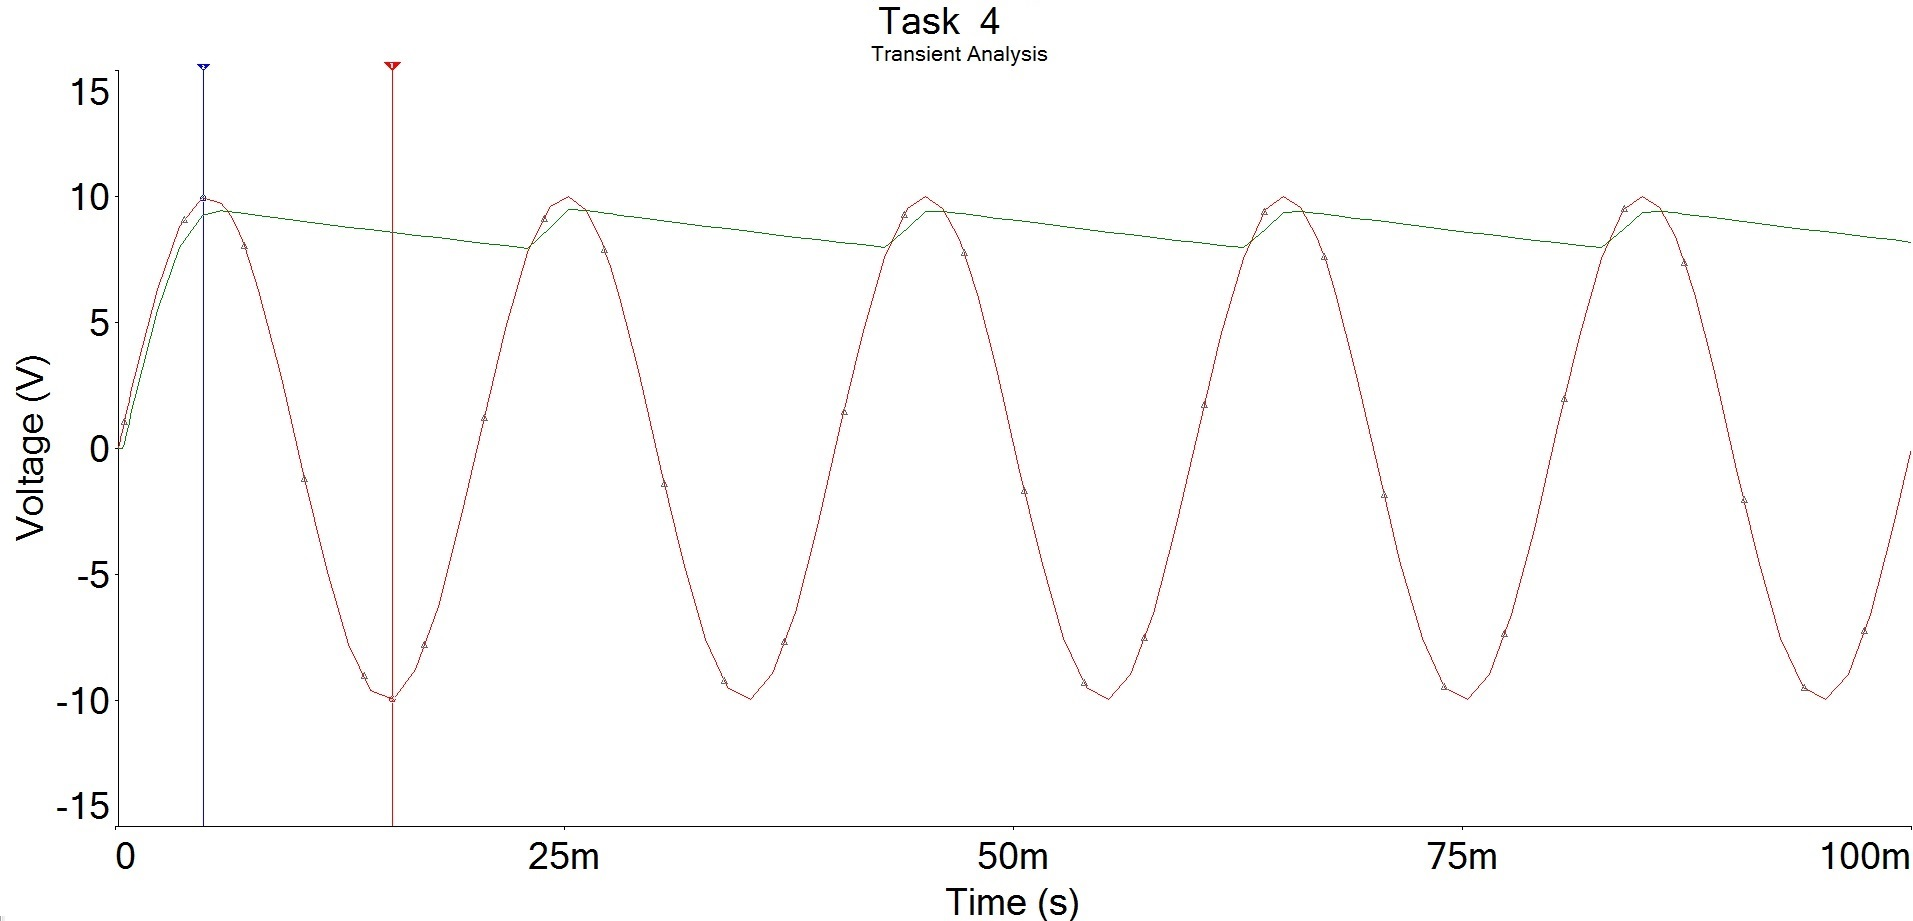
\includegraphics[width=13cm]{4_2.jpg}
    \end{minipage}


    The data for the cursors on the previous figure:\\
    
    \begin{minipage}{\linewidth}
    	\centering
		\captionof{figure}{}        
        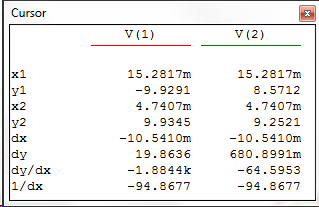
\includegraphics[width=9cm]{table_4_1.png}
    \end{minipage}
    
    \vspace{2em}
        
    So the peak voltage is y2 in the table above. That is $V_p = 9.935 V$ 
    
    The theoretical value was defined as $V_p = 10 V$ \\
    
    \begin{minipage}{\linewidth}
    	\centering
		\captionof{figure}{}        
        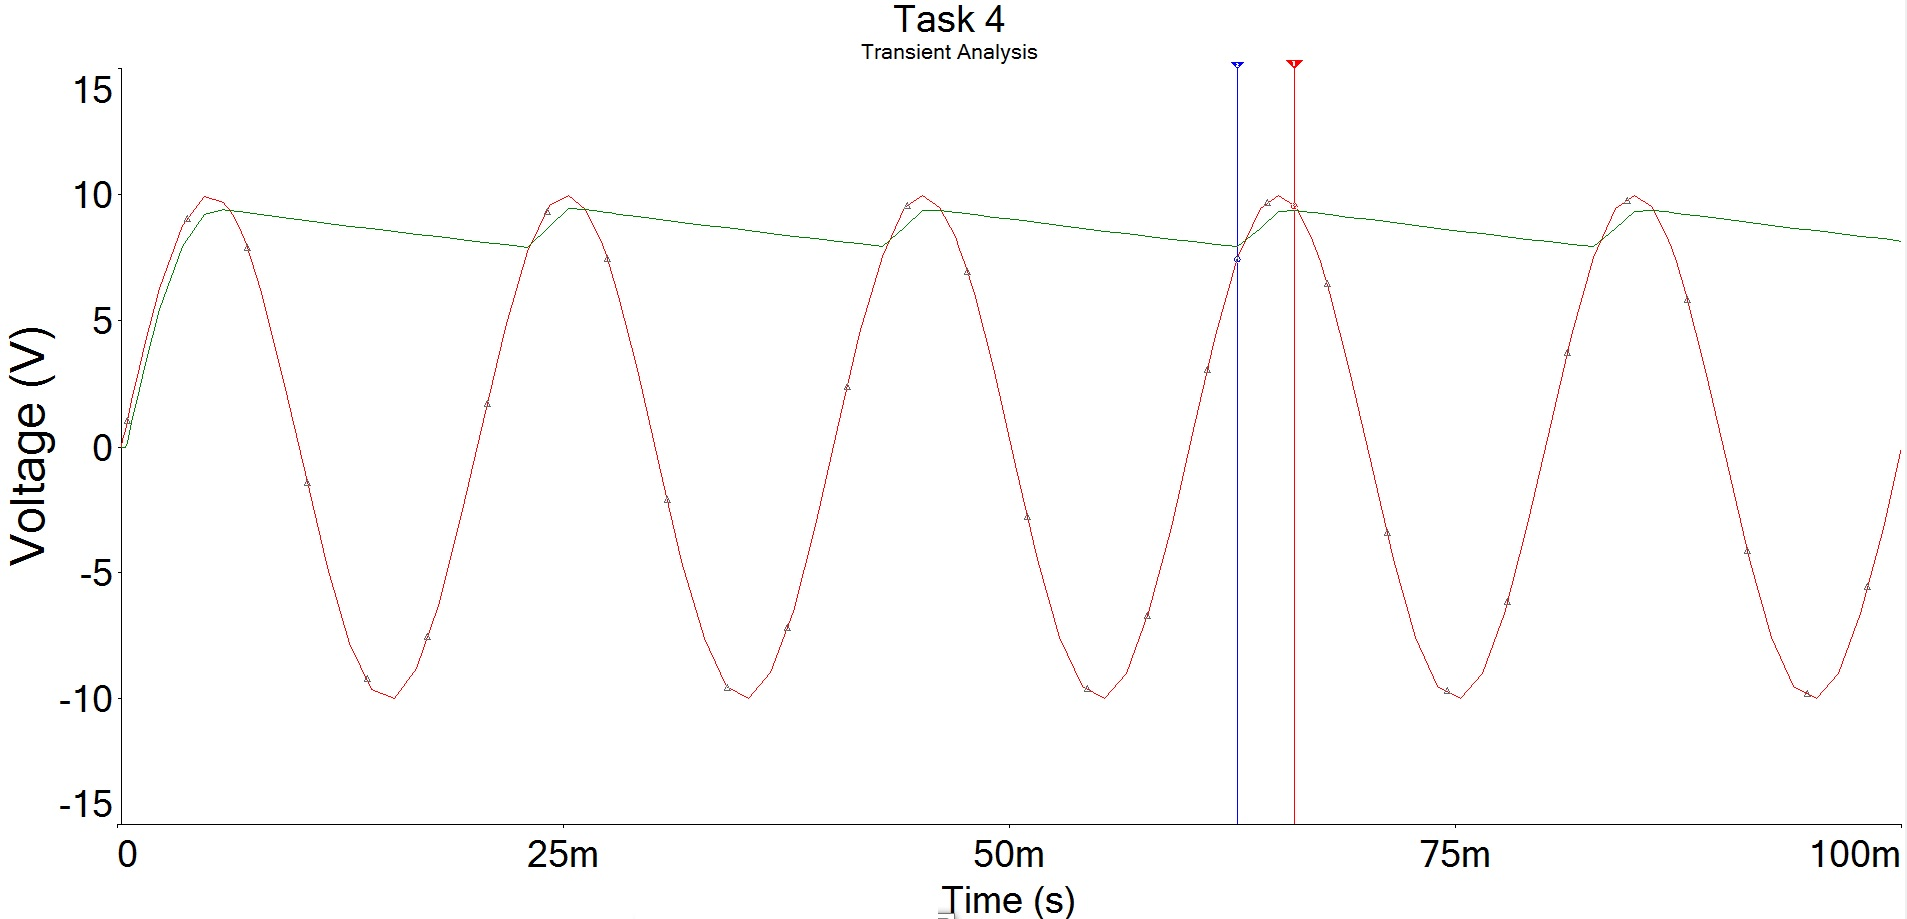
\includegraphics[width=13cm]{4_3.jpg}
    \end{minipage}
    
    \begin{minipage}{\linewidth}
    	\centering
		\captionof{figure}{}        
        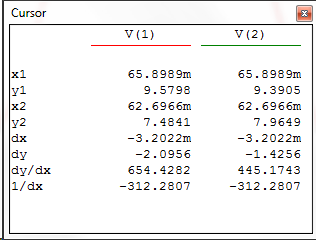
\includegraphics[width=9cm]{table_4_2.png}
    \end{minipage}
    
    \vspace{2em}
    
	The ripple voltage can be calculated from the graph. The maximum difference in voltage over the diode over one period is the ripple voltage so it can simply be seen from the graph and table, using the cursors: $$ V_r = 9.5798 V - 7.4841 V = 2.096 V$$
    The theoretical ripple voltage value can be calculated with: $$ V_r = \dfrac{V_p}{fCR} = \dfrac{10}{50 \cdot 100 \cdot 10^{-6} \cdot 10^3} = 2 V$$
    \vspace{2em}
  
  \item[$\bold{3.}$]
  
  	The ripple voltage will then be: $V_r = V_p \cdot 0.02 = 0.1987 V$. Now we can calculate the maximum value of the capacitance, C: $$ C = \dfrac{V_p}{f R V_r} = \dfrac{V_p}{f R V_p \cdot 0.02} = \dfrac{1}{f R \cdot 0.02} = \dfrac{1}{50 \cdot 10^3 \cdot 0.02} = 1mF $$
  
  \begin{minipage}{\linewidth}
    	\centering
		\captionof{figure}{The transient analysis were the capacitor value is $1mF$ instead of $100\mu F$}        
        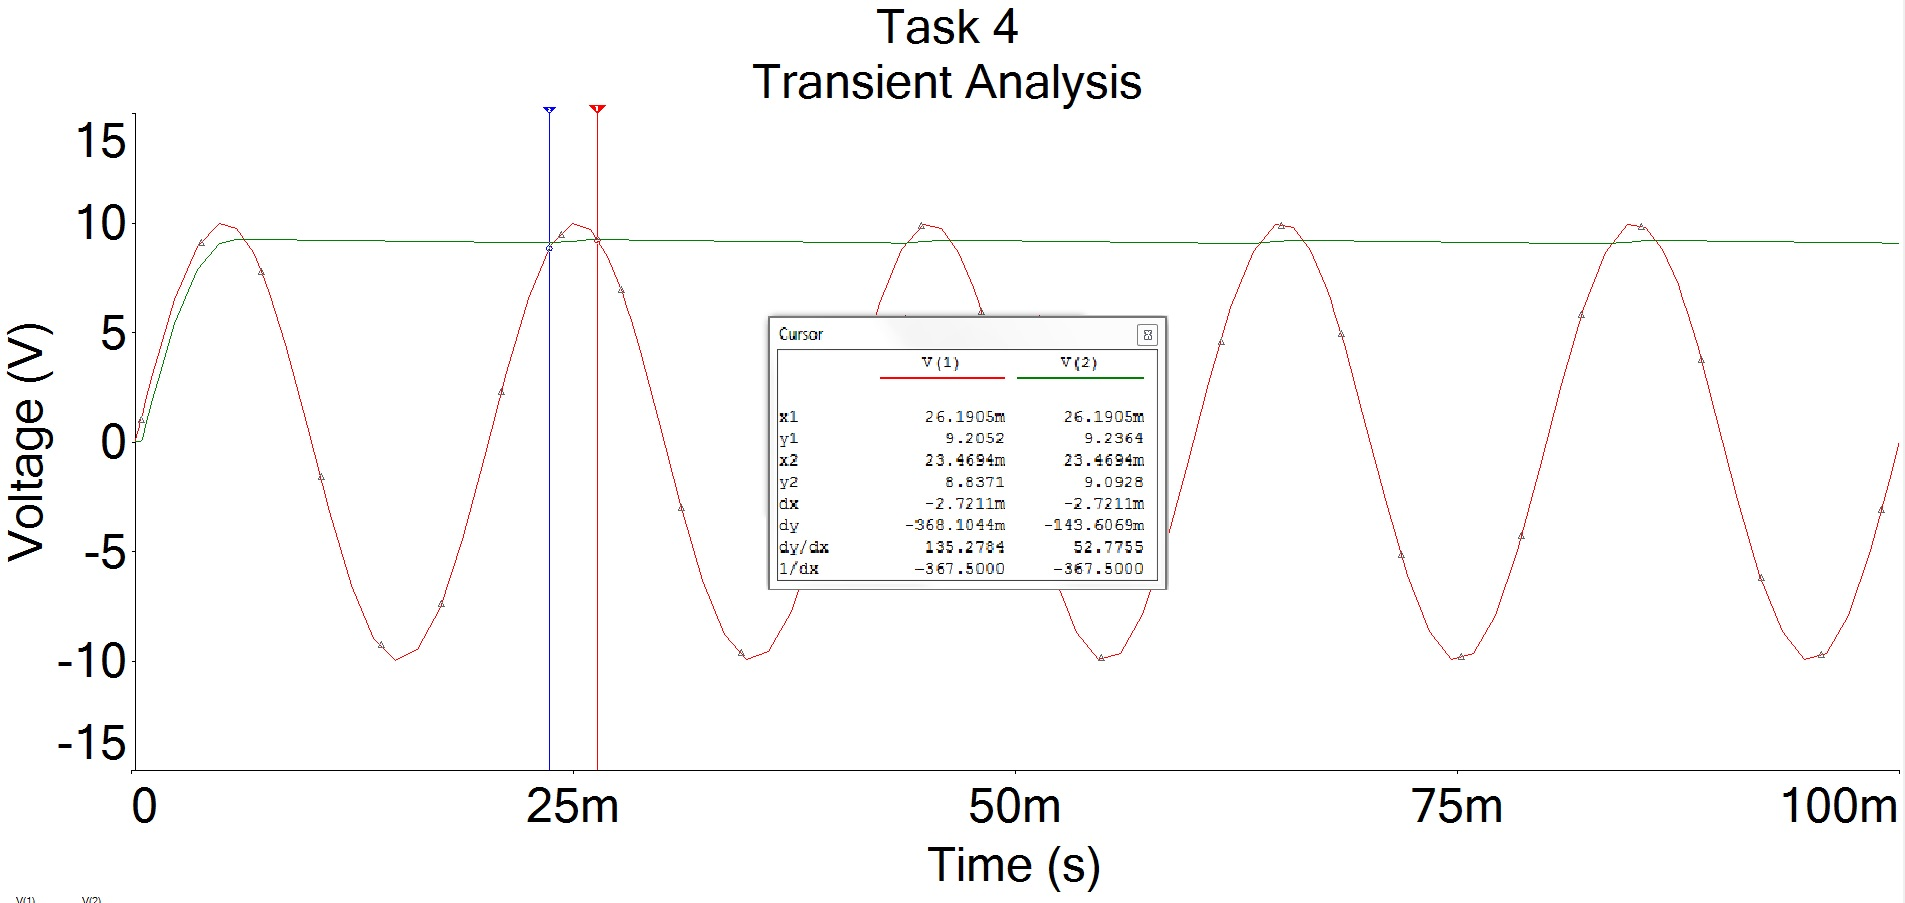
\includegraphics[width=13cm]{4_4.jpg}
  \end{minipage}
    
   The ripple voltage should not be larger than 2 $\%$ of the peak voltage, $V_r(max) = 0.02 \cdot 9.935 V = 0.1987 V$. And from the graph and cursors the actual ripple voltage after the change: $$ V_r = 9.2364 \: V - 9.0928 \: V = 0.1436 \: V < V_r(max) = 0.1987 \: V$$
   

\end{enumerate}



\end{document}
\\
